\subsection{Code overview}\label{sec:code_overview}
The C-code \ref{eis:3.3} that will manage all the data on the ODROID consists of several elements. An overview of how these elements and their data are managed can be found in \Cref{fig:code_overview}.\\

\begin{figure}[!ht]
  \centering
    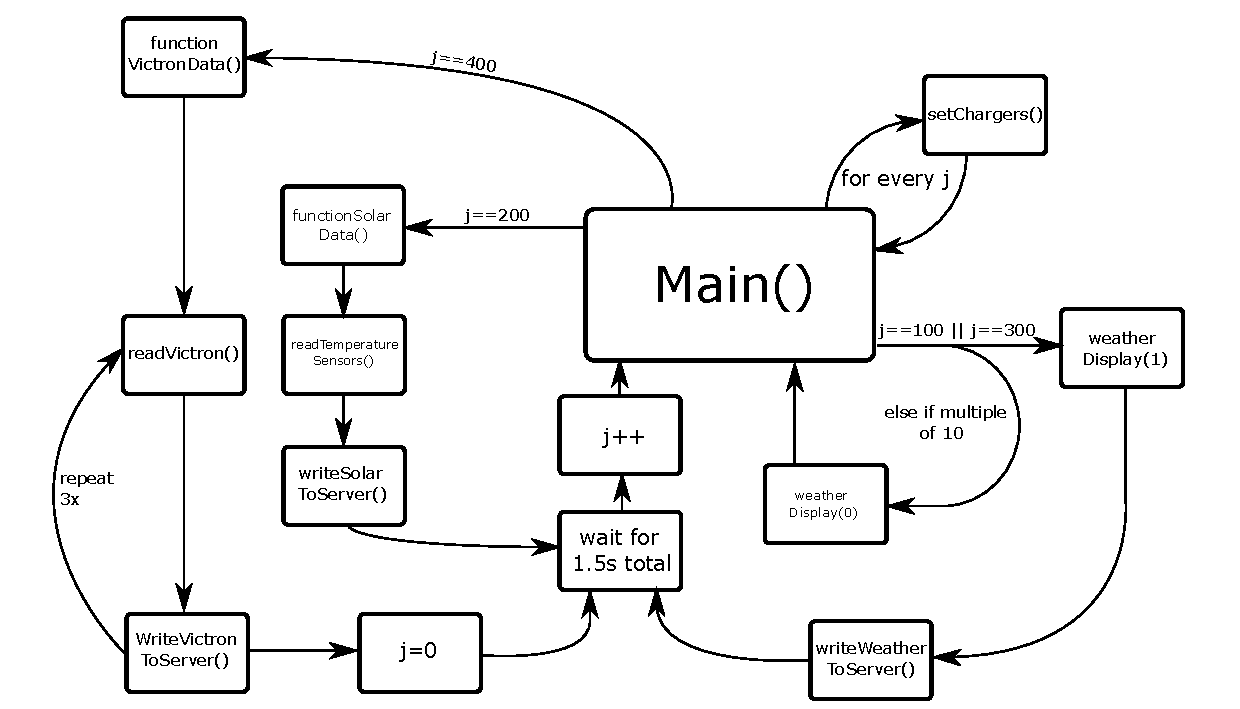
\includegraphics[width=1.0\textwidth]{images/ODROID_code_overview.pdf}
      \caption{An overview of the C code}\label{fig:code_overview}
\end{figure}

The entire program is built around a variable \verb|j| that keeps track of time by incrementing every 1.5 seconds. This variable resets to zero every time it is reaches 400, creating a loop that restarts every 10 minutes.\\

The ODROID will decide what data to handle based on this variable. For every j, the ODROID will fetch the charger states from the server and set the chargers using the \verb|setChargers()| function. Every 5 minutes (when \verb|j| equals 100 or 300), data from the weather station is fetched and sent to the server (\verb|weatherDisplay(1)|). Every 15 seconds (when \verb|j| is a multiple of 10), data will also be fetched from the weather station, but only to refresh the local display (\verb|weatherDisplay(0)|). To prevent this event from causing two data fetches to the weather station, it is only run if it does not conflict with \verb|weatherDisplay(1)| (by using \verb|else if|). Note that \verb|weatherDisplay(0)| does not increment \verb|j|, so it is possible that it runs together (before) the functions starting at \verb|j| equal to 400 or 200.\\

Every 10 minutes (when \verb|j| equals 200), data from the temperature probes is read. This data is also sent to the server. A similar loop is also run every 10 minutes (when \verb|j| equals 400) which will read the Victron data. This loop will be run 3 times because there are three seperate chunks of data that will be read (further explained in \Cref{sec:Victron}). Every chunk of data is seperately sent to the server.\\